\documentclass{bredelebeamer}

%%%%%%%%%%%%%%%%%%%%%%%%%%%%%%%%%%%%%%%%%%%%%%%%

\title[Programación en MatLAB]{Introducción a la programación con MatLAB}
\subtitle{Módulo 08 - Archivos en matlab}

\author{Autor1 - Autor2 - Autor3\inst{1}}
\institute[UTN.BA]
{
  \inst{1}%
  Universidad Tecnológica Nacional\\
  Facultad Regional Buenos Aires
  }

\date{dia mes 2018}

\subject{Taller de programación}

\logo{

\includegraphics[scale=0.15]{images/logo.png}
}

%%%%%%%%%%%%%%%%%%%%%%%%%%%%%%%%%%%%%%%%%%%%%%%%%%%%%%%%%%%%%%%%%%%%%
\begin{document}

\begin{frame}
  \titlepage 
\end{frame}

%%%%%%%%%%%%%%%%%%%%%%%%%%%%%%%%%%%%%%%%%%%%%%%%%%%%%%%%%%%%%%%%%%%%%

% Archivos

%%%%%%%%%%%%%%%%%%%%%%%%%%%%%%%%%%%%%%%%%%%%%%%%%%%%%%%%%%%%%%%%%%%%%
\section{Archivos en Matlab}

\begin{frame}{Importación de datos}
Los datos se almacenan en muchos formatos diferentes. Algunos ejemplos podrían ser:
\begin{itemize}
\item Sonido: se almacena en un archivo .wav
\item Imagen: archivos .jpg
\item Tablas de excel: .xls
\end{itemize}
Para conocer los formatos admitidos por MATLAB escribir \textbf{doc fileformats} en la ventana de comandos.
\end{frame}

\begin{frame}{Tipos de archivo soportados por Matlab}
Matlab soporta los siguientes tipos de archivo de datos
\begin{table}[]
\centering
\begin{tabular}{|c|c|c|}
\hline
Tipo de archivo                                                                  & Extensión                                                         & Observación                                                                                                             \\ \hline
Texto                                                                            & \begin{tabular}[c]{@{}c@{}}.mat\\ .dat\\ .txt\end{tabular}        & \begin{tabular}[c]{@{}c@{}}Area de trabajo matlab\\ Datos ASCII\\ Datos ASCII\end{tabular}                              \\ \hline
\begin{tabular}[c]{@{}c@{}}Formatos comunes \\ de datos científicos\end{tabular} & \begin{tabular}[c]{@{}c@{}}.cdf\\ .fits\\ .hdf\end{tabular}       & \begin{tabular}[c]{@{}c@{}}Datos comunes\\ Transporte de imágenes\\ Datos jerárquicos\end{tabular}                      \\ \hline
Datos de hoja de cálculo                                                         & \begin{tabular}[c]{@{}c@{}}.xls\\ .wk1\\ .tiff\end{tabular}       & \begin{tabular}[c]{@{}c@{}}Hoja de cálculo Excel\\ Lotus 123\\ Archivo de imagen etiquetado\end{tabular}                \\ \hline
Datos de imágen                                                                  & \begin{tabular}[c]{@{}c@{}}.bmp\\ .jpeg o jpg\\ .gif\end{tabular} & \begin{tabular}[c]{@{}c@{}}Mapa de bits\\ Grupo experto fotográfico unido\\ Formato de intercambio gráfico\end{tabular} \\ \hline
Datos de audio                                                                   & \begin{tabular}[c]{@{}c@{}}.au\\ .wav\end{tabular}                & \begin{tabular}[c]{@{}c@{}}Audio\\ Archivo wave Microsoft\end{tabular}                                                  \\ \hline
Película                                                                         & .avi                                                              & Archivo intercalado audio/video                                                                                         \\ \hline
\end{tabular}
\end{table}
\end{frame}

\begin{frame}{Importación de datos}
Conociendo el tipo de formato a importar puede utilizar una función de importación. Por ejemplo:
\boiteviolette{
[data,fs] = wavread('ArrozConLeche.wav');
}
Lee la canción \textit{ArrozConLeche}\\
\begin{block}{Tener en cuenta}
\textbf{doc fileformats} muestra una lista de funciones de importación según el formato del archivo a importar.
\end{block}
\end{frame}

\begin{frame}{Cargar datos desde un archivo ASCII}
\begin{itemize}
\item Un archivo ASCII contiene datos como texto
\item Todas las filas contienen el mismo número de datos.
\end{itemize}
Un ejemplo de archivo \textbf{text.txt} puede ser:
\begin{table}[]
\centering
\begin{tabular}{cccc}
\multicolumn{4}{c}{texto.txt} \\
2.5   & 7      & -3.2  & 4    \\
5     & 2.1    & 3.7   & 12   \\
-2    & -0.3   & 37    & -19  \\
4     & 3.2    & -1    & 0   
\end{tabular}
\end{table}
\begin{exampleblock}{Comando}
Ver comando: \textbf{load()}
\end{exampleblock}
Para cargar el archivo \textit{texto.txt} se escribe:\\
\boiteviolette{
variable = load(’texto.txt’);
}
\end{frame}

\begin{frame}{Función textread}
\begin{itemize}
\item Lee string y datos numéricos desde un archivo utilizando especificadores de conversión.
\item Los especificadores de conversión son por ejemplo formato de datos.
\item La función es útil cuando el archivo tiene un formato uniforme.
\end{itemize}
Un ejemplo de archivo \textbf{text.txt} puede ser:
\begin{table}[]
\centering
\begin{tabular}{cccc}
\multicolumn{4}{c}{texto.txt} \\
2.5   & 7      & -3.2  & 4    \\
5     & 2.1    & 3.7   & 12   \\
-2    & -0.3   & 37    & -19  \\
4     & 3.2    & -1    & 0   
\end{tabular}
\end{table}
\begin{exampleblock}{Comando}
Ver comando: \textbf{textread()}
\end{exampleblock}
Para cargar el archivo \textit{texto.txt} se escribe:\\
\boiteviolette{
variable = textread(’texto.txt’);
}
\end{frame}

\begin{frame}{Función textread}
Para leer un archivo \textbf{.dat}. Por ejemplo:
\begin{table}[]
\centering
\begin{tabular}{cccc}
\multicolumn{4}{c}{personas.dat} \\
Manuel     & Hombre & 20 & Mayor \\
Camila     & Mujer  & 19 & Mayor \\
Juan       & Hombre & 33 & Mayor \\
Florencia  & Mujer  & 14 & Menor
\end{tabular}
\end{table}
\begin{block}{Formato}
\begin{center}
[A,B,C, ...] = textread(’archivo’,’formato’,N)\\
N es el número de filas que se deseen leer. El valor -1 permite leer todo el archivo.
\end{center}
\end{block}
Para cargar el archivo \textit{personas.dat} se escribe:\\
\boiteviolette{
[nombre, tipo,edad,estado]=textread(’misdatos.dat’, ’\%s \%s \%f \%s’, -1)
}
\end{frame}

\begin{frame}{Función dlmread}
\begin{exampleblock}{Comando}
Ver comando: \textbf{dlmread()}
\end{exampleblock}
La función \textbf{dlmread} permite leer una lista de valores desde un archivo separado por delimitadores.\\
Ej. Leer la siguiente tabla de datos separados por \textbf{;}
\begin{table}[]
\centering
\begin{tabular}{cccc}
\multicolumn{4}{c}{signal.dat} \\
4;     & 3;     & 2.4;  & 7    \\
-3;    & 0.33;  & 20;   & 12   \\
1;     & 1.7;   & 9;    & 12.4 \\
0.33;  & 9.3;   & -2;   & 3.3 
\end{tabular}
\end{table}
\boiteviolette{
datos=dlmear(’signal.dat’, ’;’);
}
\end{frame}

\begin{frame}{Función xlsread}
\begin{exampleblock}{Comando}
Ver comando: \textbf{xlsread()}
\end{exampleblock}
\begin{itemize}
\item xlsread lee una hoja de cálculo de formato excel (xls)
\item Las celdas vacías o de texto serán retornadas como NaN en el dato
\end{itemize}
Ej. Leer la siguiente tabla de datos
\begin{table}[]
\centering
\begin{tabular}{cccc}
\multicolumn{4}{c}{datos.xls}                                                                                    \\ \hline
\multicolumn{1}{|c|}{4}    & \multicolumn{1}{c|}{3}    & \multicolumn{1}{c|}{2.4} & \multicolumn{1}{c|}{7}    \\ \hline
\multicolumn{1}{|c|}{-3}   & \multicolumn{1}{c|}{0.33} & \multicolumn{1}{c|}{20}  & \multicolumn{1}{c|}{12}   \\ \hline
\multicolumn{1}{|c|}{1}    & \multicolumn{1}{c|}{1.7}  & \multicolumn{1}{c|}{9}   & \multicolumn{1}{c|}{12.4} \\ \hline
\multicolumn{1}{|c|}{0.33} & \multicolumn{1}{c|}{9.3}  & \multicolumn{1}{c|}{-2}  & \multicolumn{1}{c|}{3.3}  \\ \hline
\end{tabular}
\end{table}
\boiteviolette{
datos=xlsread(’datos.xls’)
}
\end{frame}

\begin{frame}{Función xlsread}
Ej. Leer la siguiente tabla de datos
\begin{table}[]
\centering
\begin{tabular}{cccc}
\multicolumn{4}{c}{datos.xls}                                                                                              \\ \hline
\multicolumn{1}{|c|}{Canal 1} & \multicolumn{1}{c|}{Canal 2} & \multicolumn{1}{c|}{Canal 3} & \multicolumn{1}{c|}{Canal 4} \\ \hline
\multicolumn{1}{|c|}{4}      & \multicolumn{1}{c|}{3}      & \multicolumn{1}{c|}{2.4}    & \multicolumn{1}{c|}{7}       \\ \hline
\multicolumn{1}{|c|}{-3}     & \multicolumn{1}{c|}{0.33}   & \multicolumn{1}{c|}{20}     & \multicolumn{1}{c|}{12}      \\ \hline
\multicolumn{1}{|c|}{1}      & \multicolumn{1}{c|}{1.7}    & \multicolumn{1}{c|}{9}      & \multicolumn{1}{c|}{12.4}    \\ \hline
\multicolumn{1}{|c|}{0.33}   & \multicolumn{1}{c|}{9.3}    & \multicolumn{1}{c|}{-2}     & \multicolumn{1}{c|}{3.3}     \\ \hline
\end{tabular}
\end{table}
\boiteviolette{
[datos,canales]=xlsread(’datos.xls’);
}
\end{frame}

\begin{frame}{Exportación de datos}
Se verán tres formas de exportar datos:\\
\begin{itemize}
\item Función save - Salva el espacio de trabajo (workspace)
\item Función dlmwrite - Guarda un arreglo utilizando delimitadores
\item Función xlswrite - Guarda un arreglo en una hoja de excel
\end{itemize}
\end{frame}

\begin{frame}{Función save}
\begin{exampleblock}{Comando}
Ver comando: \textbf{save}
\end{exampleblock}
La función \textbf{save} guarda el espacio de trabajo (workspace) en forma binaria creando un archivo .mat
\begin{exampleblock}{Comando}
Ver comando: \textbf{load}
\end{exampleblock}
La función \textbf{load} carga el archivo .mat recuperando el workspace salvado.
\begin{block}{Tener en cuenta}
\begin{center}
Para guardar el workspace con un determinado nombre se escribe:\\
filename = 'test.mat';\\
save(filename);
\end{center}
\end{block}
\end{frame}

\begin{frame}{Función save}
Ej. Ejecutar las siguientes líneas. Obtener conclusiones.
\boiteviolette{
A = 5;\\
B = 6;\\
espacio = 'espacioTrabajo';\\
save(espacio);\\
clear;\\
load('espacioTrabajo.mat');
}
\end{frame}

\begin{frame}{Función dlmwrite}
\begin{exampleblock}{Comando}
Ver comando: \textbf{dlmwrite}
\end{exampleblock}
La función \textbf{dlmwrite} escribe el arreglo en un archivo delimitado por ASCII
\begin{exampleblock}{Comando}
Ver comando: \textbf{type}
\end{exampleblock}
La función \textbf{type} visualiza el archivo .txt
\end{frame}

\begin{frame}{Función dlmwrite}
Ej. Ejecutar las siguientes líneas. Obtener conclusiones.
\boiteviolette{
Matriz = magic(3);\\
dlmwrite('Archivo.txt',Matriz,'\&');\\
type('archivo.txt');
}
Ej. Ejecutar las siguientes líneas. Obtener conclusiones.
\boiteviolette{
Matriz = magic(3);\\
dlmwrite('Archivo.dat',Matriz,'\&');\\
load('archivo.txt');
}
\end{frame}

\begin{frame}{Función xlswrite}
\begin{exampleblock}{Comando}
Ver comando: \textbf{xlswrite}
\end{exampleblock}
La función \textbf{xlswrite} Guarda arreglo numérico o matriz en una hoja de Excel.

Ej. Ejecutar las siguientes líneas. Obtener conclusiones.
\boiteviolette{
Archivo = 'PrimeraTabla';\\
Matriz = [1 2 3 4 ; 5 6 7 8 ; 9 10 11 12];\\
xlswrite(Archivo,Matriz);
}
\end{frame}

%%%%%%%%%%%%%%%%%%%%%%%%%%%%%%%%%%%%%%%%%%%%%%%%%%%%%%%%%%%%%%%%%%%%%

% Sección de consultas

%%%%%%%%%%%%%%%%%%%%%%%%%%%%%%%%%%%%%%%%%%%%%%%%%%%%%%%%%%%%%%%%%%%%%

\section{Consultas}
\begin{frame}{Consultas}
\begin{center}

\includegraphics[scale=0.3]{images/consultas.png}
\end{center}
\end{frame}


%%%%%%%%%%%%%%%%%%%%%%%%%%%%%%%%%%%%%%%%%%%%%%%%%%%%%%%%%%%%%%%%%%%%%

% Sección de bibliografía

%%%%%%%%%%%%%%%%%%%%%%%%%%%%%%%%%%%%%%%%%%%%%%%%%%%%%%%%%%%%%%%%%%%%%

\section{Bibliografia}

\begin{frame}{Bibliografía}
\begin{columns}
\begin{column}{0.5\textwidth}
\begin{center}

\includegraphics[scale=0.4]{images/biblio1.png}
\end{center}
\end{column}
\begin{column}{0.5\textwidth}
\begin{center}
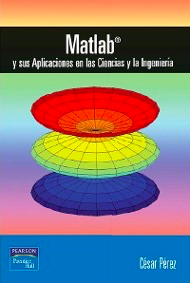
\includegraphics[scale=0.5]{images/biblio2.png}
\end{center}
\end{column}
\end{columns}
\end{frame}

\end{document}
